\begin{figure*}[t!]
    \centering
    \begin{subfigure}[b]{0.22\linewidth}
        \centering
        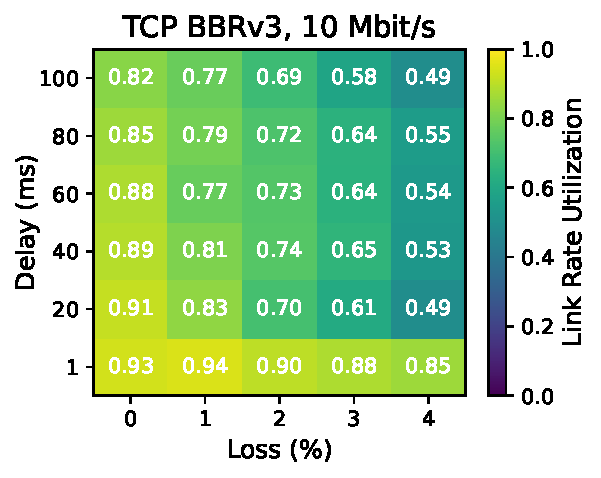
\includegraphics[width=\linewidth,trim={0 0 2cm 0.7cm},clip]
        {splitting-paper/figures/heatmaps/heatmap_tcp_bbr3_10mbps.pdf}
        \captionsetup{skip=4pt}
        \caption{TCP, BBRv3}
        \label{fig:quic:tcp-bbr3}
    \end{subfigure}
    \begin{subfigure}[b]{0.22\linewidth}
        \centering
        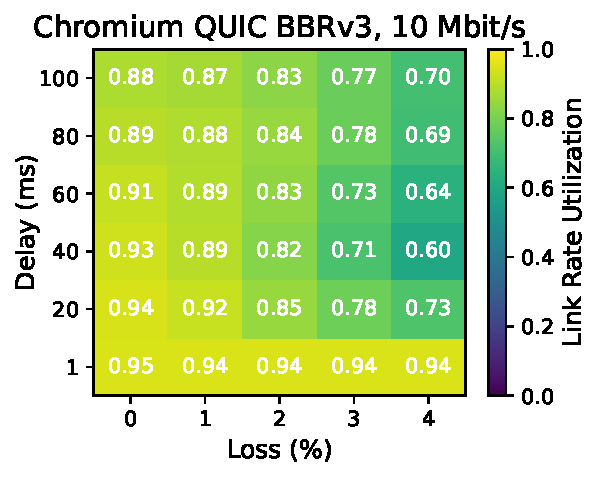
\includegraphics[width=\linewidth,trim={0 0 2cm 0.7cm},clip]
        {splitting-paper/figures/heatmaps/heatmap_quic_bbr3_10mbps.pdf}
        \captionsetup{skip=4pt}
        \caption{Google \texttt{quiche}, BBRv3}
        \label{fig:quic:google-bbr3}
    \end{subfigure}
    \begin{subfigure}[b]{0.22\linewidth}
        \centering
        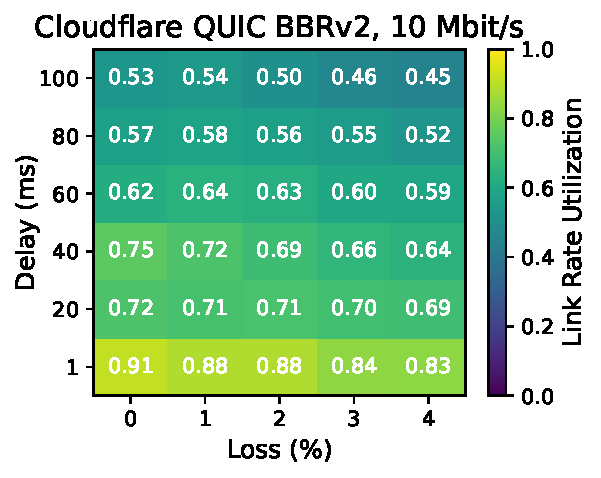
\includegraphics[width=\linewidth,trim={0 0 2cm 0.7cm},clip]
        {splitting-paper/figures/heatmaps/heatmap_quiche_bbr2_10mbps.pdf}
        \captionsetup{skip=4pt}
        \caption{Cloudflare \texttt{quiche}, BBRv2}
        \label{fig:quic:cloudflare-bbr2}
    \end{subfigure}
    \begin{subfigure}[b]{0.22\linewidth}
        \centering
        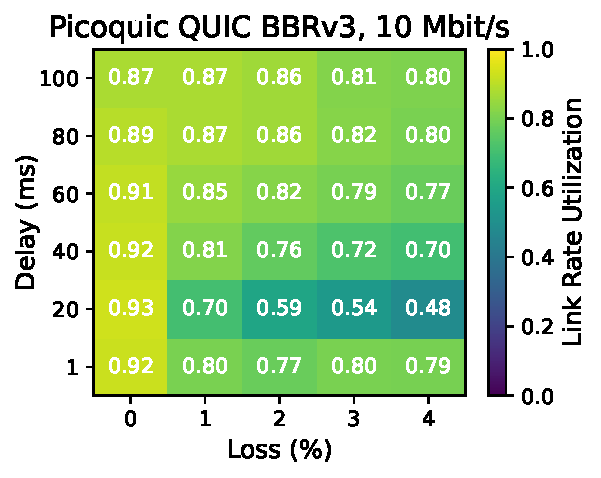
\includegraphics[width=\linewidth,trim={0 0 2cm 0.7cm},clip]
        {splitting-paper/figures/heatmaps/heatmap_picoquic_bbr3_10mbps.pdf}
        \captionsetup{skip=4pt}
        \caption{\texttt{picoquic}, BBRv3}
        \label{fig:quic:picoquic-bbr3}
    \end{subfigure}
    \begin{subfigure}[b]{1cm}
        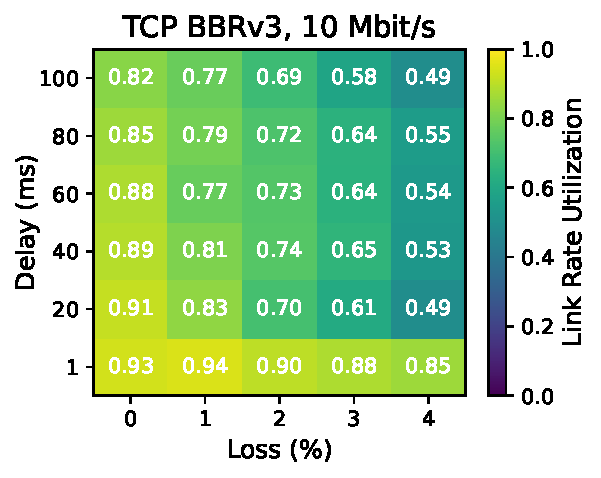
\includegraphics[width=1cm,trim={8cm 0 0 0},clip]
        {splitting-paper/figures/heatmaps/heatmap_tcp_bbr3_10mbps.pdf}
        \vspace*{0.2cm}
    \end{subfigure}
    
    \begin{subfigure}[b]{0.22\linewidth}
        \centering
        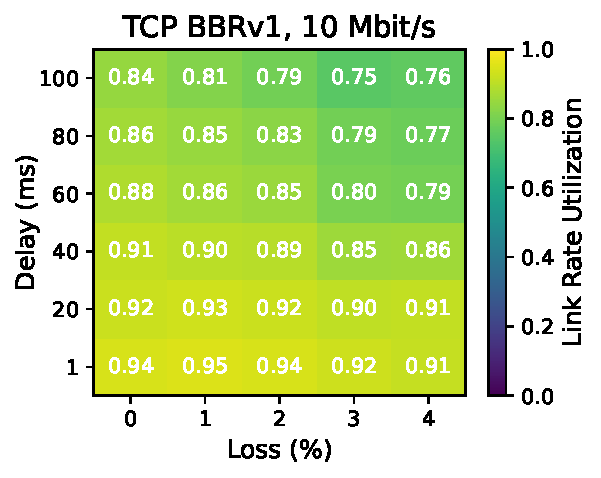
\includegraphics[width=\linewidth,trim={0 0 2cm 0.7cm},clip]
        {splitting-paper/figures/heatmaps/heatmap_tcp_bbr1_10mbps.pdf}
        \captionsetup{skip=4pt}
        \caption{TCP, BBRv1}
        \label{fig:quic:tcp-bbr1}
    \end{subfigure}
    \begin{subfigure}[b]{0.22\linewidth}
        \centering
        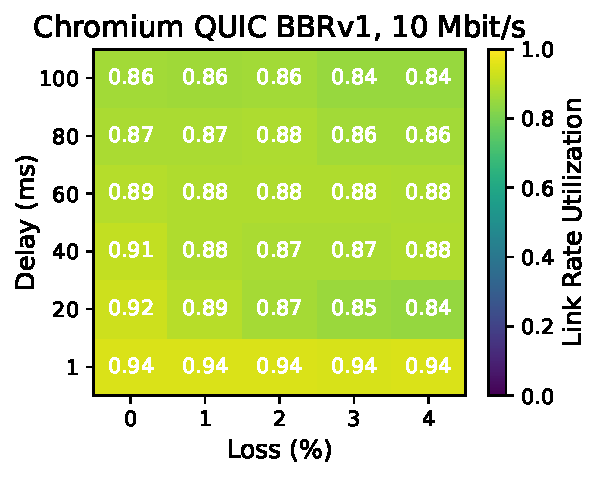
\includegraphics[width=\linewidth,trim={0 0 2cm 0.7cm},clip]
        {splitting-paper/figures/heatmaps/heatmap_quic_bbr1_10mbps.pdf}
        \captionsetup{skip=4pt}
        \caption{Google \texttt{quiche}, BBRv1}
        \label{fig:quic:google-bbr1}
    \end{subfigure}
    \begin{subfigure}[b]{0.22\linewidth}
        \centering
        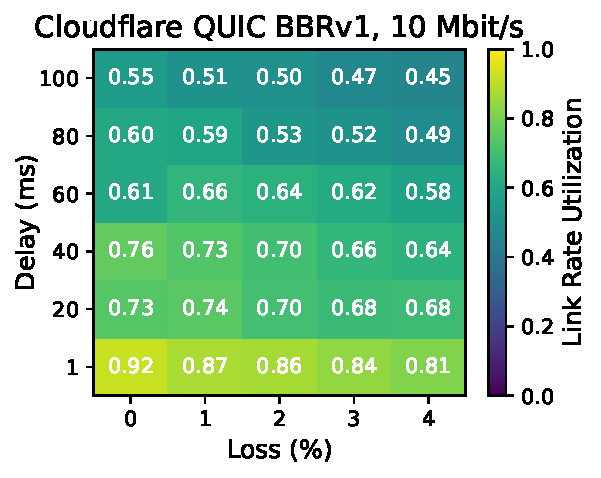
\includegraphics[width=\linewidth,trim={0 0 2cm 0.7cm},clip]
        {splitting-paper/figures/heatmaps/heatmap_quiche_bbr1_10mbps.pdf}
        \captionsetup{skip=4pt}
        \caption{Cloudflare \texttt{quiche}, BBRv1}
        \label{fig:quic:cloudflare-bbr1}
    \end{subfigure}
    \begin{subfigure}[b]{0.22\linewidth}
        \centering
        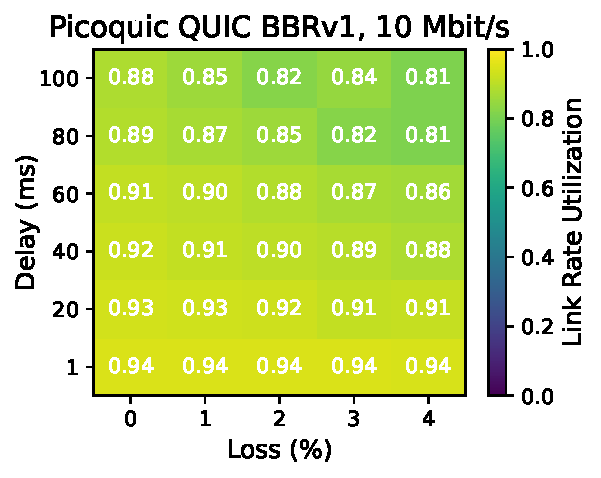
\includegraphics[width=\linewidth,trim={0 0 2cm 0.7cm},clip]
        {splitting-paper/figures/heatmaps/heatmap_picoquic_bbr1_10mbps.pdf}
        \captionsetup{skip=4pt}
        \caption{\texttt{picoquic}, BBRv1}
        \label{fig:quic:picoquic-bbr1}
    \end{subfigure}
    \begin{subfigure}[b]{1cm}
        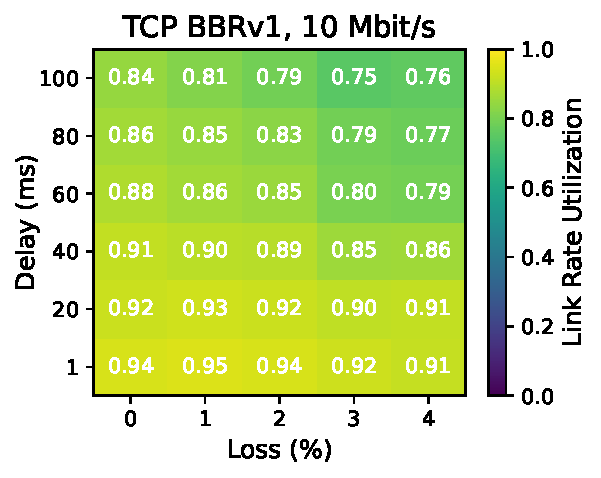
\includegraphics[width=1cm,trim={8cm 0 0 0},clip]
        {splitting-paper/figures/heatmaps/heatmap_tcp_bbr1_10mbps.pdf}
        \vspace*{0.2cm}
    \end{subfigure}

    \begin{subfigure}[b]{0.22\linewidth}
        \centering
        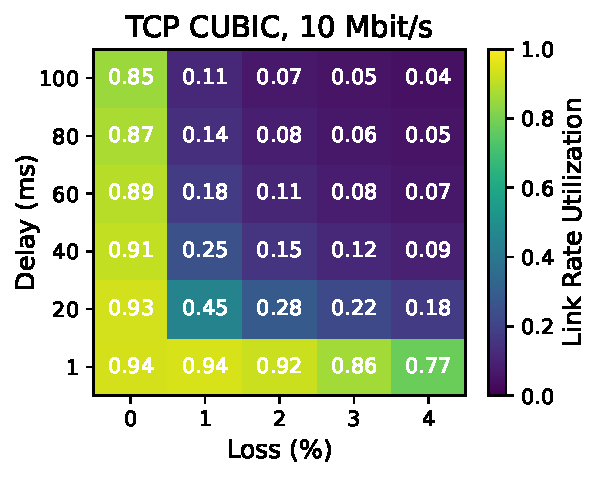
\includegraphics[width=\linewidth,trim={0 0 2cm 0.7cm},clip]
        {splitting-paper/figures/heatmaps/heatmap_tcp_cubic_10mbps.pdf}
        \captionsetup{skip=4pt}
        \caption{TCP, CUBIC}
        \label{fig:quic:tcp-cubic}
    \end{subfigure}
    \begin{subfigure}[b]{0.22\linewidth}
        \centering
        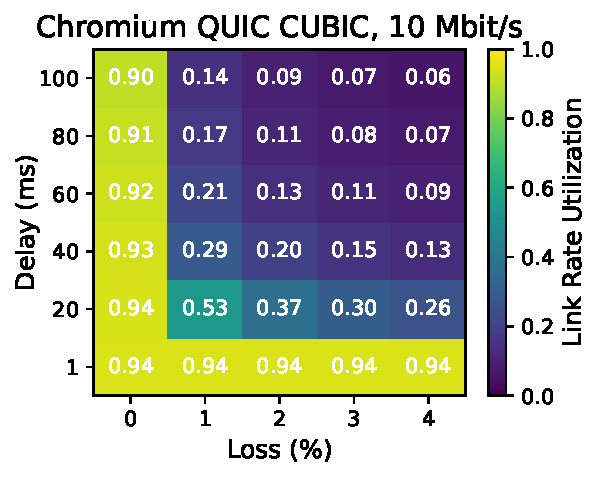
\includegraphics[width=\linewidth,trim={0 0 2cm 0.7cm},clip]
        {splitting-paper/figures/heatmaps/heatmap_quic_cubic_10mbps.pdf}
        \captionsetup{skip=4pt}
        \caption{Google \texttt{quiche}, CUBIC}
        \label{fig:quic:google-cubic}
    \end{subfigure}
    \begin{subfigure}[b]{0.22\linewidth}
        \centering
        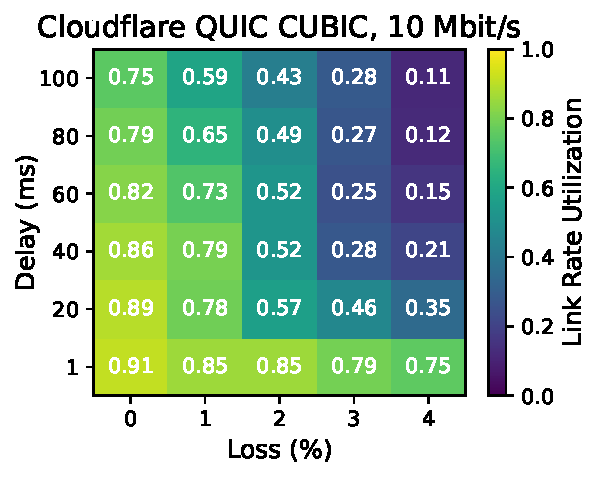
\includegraphics[width=\linewidth,trim={0 0 2cm 0.7cm},clip]
        {splitting-paper/figures/heatmaps/heatmap_quiche_cubic_10mbps.pdf}
        \captionsetup{skip=4pt}
        \caption{Cloudflare \texttt{quiche}, CUBIC}
        \label{fig:quic:cloudflare-cubic}
    \end{subfigure}
    \begin{subfigure}[b]{0.22\linewidth}
        \centering
        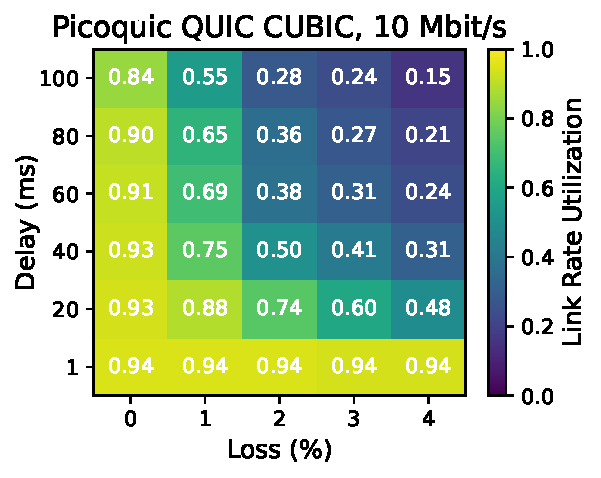
\includegraphics[width=\linewidth,trim={0 0 2cm 0.7cm},clip]
        {splitting-paper/figures/heatmaps/heatmap_picoquic_cubic_10mbps.pdf}
        \captionsetup{skip=4pt}
        \caption{\texttt{picoquic}, CUBIC}
        \label{fig:quic:picoquic-cubic}
    \end{subfigure}
    \begin{subfigure}[b]{1cm}
        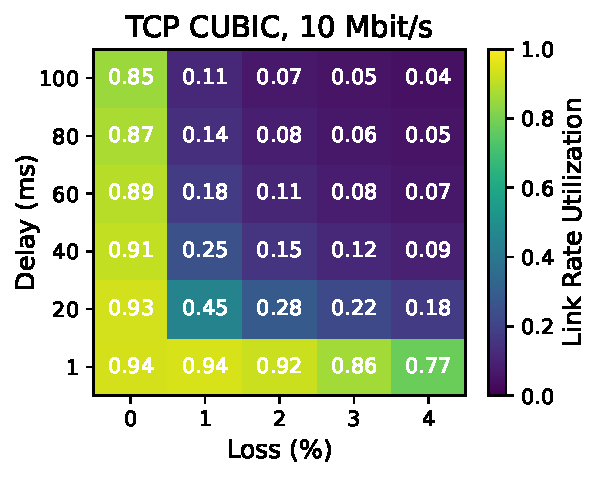
\includegraphics[width=1cm,trim={8cm 0 0 0},clip]
        {splitting-paper/figures/heatmaps/heatmap_tcp_cubic_10mbps.pdf}
        \vspace*{0.2cm}
    \end{subfigure}

    \caption{Heatmaps for three QUIC implementations of BBRv3 (or BBRv2), BBRv1,
     and CUBIC showing link rate utilization calculated as the ratio of
     achieved goodput to link rate, compared to Linux TCP. The heatmaps are
     shown at various loss rates and one-way delays with a fixed link rate of
     10 Mbit/s. User-space QUIC is not CPU-limited, achieving high utilizations
     at 1 ms delay and 0\% loss. The QUIC implementations are Google \texttt
     {quiche}, Cloudflare \texttt{quiche}, and a minimalist implementation
     based on the IETF spec called \texttt{picoquic}. Median of $n=20$
     trials.}
    \label{fig:quic}
    \vspace{-0.3cm}
\end{figure*}
